%\vspace{1.5\baselineskip}
\begin{figure}[H]
    \begin{center}
        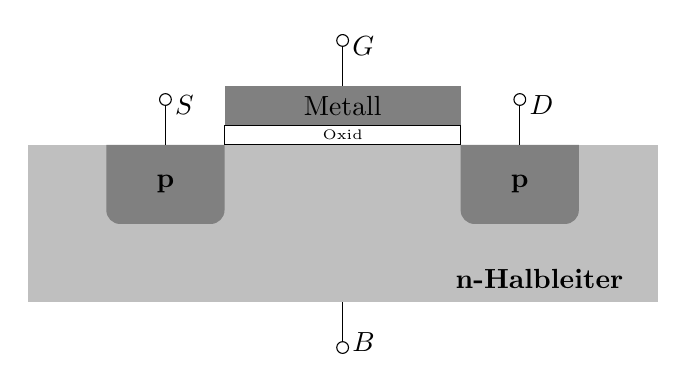
\begin{tikzpicture}
            % N-Type Substrate
            \fill[lightgray] (-4,1) rectangle (4,-1);
            \node at (2.5,-.7) {\textbf{n-Halbleiter}};
            
            % P+ regions
            \fill[gray]
                (-3,1) -- (-1.5,1) -- 
                ++(0,-0.83) arc[start angle=0, end angle=-90, radius=5pt] -- 
                ++(-1.15,0) arc[start angle=-90, end angle=-180, radius=5pt] -- 
                cycle;
            \node at (-2.25,0.5) {\textbf{p}};
            \fill[gray]
                (1.5,1) -- (3,1) -- 
                ++(0,-0.83) arc[start angle=0, end angle=-90, radius=5pt] -- 
                ++(-1.15,0) arc[start angle=-90, end angle=-180, radius=5pt] -- 
                cycle;
            \node at (2.25,0.5) {\textbf{p}};

            % Gate
            \fill[gray]
                (-1.5,1.75) rectangle (1.5,1.25);
            \node at (0,1.5) {{Metall}};
            \draw (-1.5,1.25) rectangle (1.5,1)
                node at (0,1.125) {\tiny{Oxid}};
            \draw (0,1.75) -- ++(0,0.5)   
                node[circle, draw,inner sep=1.5pt] at (0,2.325){}
                    node[right]{$G$};

            % Source 
            \draw (-2.25,1) -- ++(0,0.5)   
                node[circle, draw,inner sep=1.5pt] at (-2.25,1.575){}
                    node[right]{$S$};
                    
            % Drain 
            \draw (2.25,1) -- ++(0,0.5)   
                node[circle, draw,inner sep=1.5pt] at (2.25,1.575){}
                    node[right]{$D$};

            % Bulk
            \draw (0,-1) -- ++(0,-0.5)   
                node[circle, draw,inner sep=1.5pt] at (0,-1.575){}
                    node[right]{$B$};
                    
        \end{tikzpicture}
    \end{center}
    \caption[Struktur PMOS-Transistor]{\\Quelle: Eigene Darstellung Struktur PMOS-Transistor in Anlehnung an \cite[S. 107]{Göbel2019}}
    \label{fig:pmos_structure}
\end{figure}
% \vspace{1.5\baselineskip}